\documentclass[aspectratio=169,11pt]{beamer}

% Theme and colors
\usetheme{Madrid}
\usecolortheme{whale}
\setbeamertemplate{navigation symbols}{}
\setbeamertemplate{footline}[frame number]

% Packages
\usepackage[utf8]{inputenc}
\usepackage[T1]{fontenc}
\usepackage{graphicx}
\usepackage{booktabs}
\usepackage{amsmath}
\usepackage{hyperref}
\usepackage{tikz}
\usetikzlibrary{shapes,arrows,positioning,calc,fit,backgrounds,decorations.pathmorphing,patterns}
\usepackage{siunitx}
\usepackage{xcolor}
\usepackage{array}
\usepackage{listings}

% Listing style for code
\lstset{
    basicstyle=\ttfamily\scriptsize,
    breaklines=true,
    frame=single,
    backgroundcolor=\color{gray!10},
    keywordstyle=\color{blue!70},
    commentstyle=\color{green!50!black},
    stringstyle=\color{red!60},
    showstringspaces=false,
    tabsize=2
}

% Custom colors
\definecolor{questionbg}{RGB}{255,248,220}
\definecolor{questionborder}{RGB}{255,193,7}
\definecolor{solutionbg}{RGB}{220,255,220}
\definecolor{solutionborder}{RGB}{40,167,69}

% Title information
\title[EECE5155 -- Cloud Pipeline Exercises]{Practical Exercises: IoT Cloud Data Pipeline}
\subtitle{Modules 6--8: MQTT, Storage, and Analytics with Real Data}
\author{Eduardo Baena}
\date{Spring 2026}
\institute{Northeastern University\\Department of Electrical and Computer Engineering\\
\texttt{e.baena@northeastern.edu}}

\begin{document}

% Title slide
\begin{frame}
    \titlepage
    \vspace{-1cm}
    \begin{center}
        \textbf{EECE5155: Wireless Sensor Networks and the Internet of Things}
    \end{center}
\end{frame}

% Overview
\begin{frame}{Exercise Overview}
    \textbf{These exercises give you hands-on experience with the IoT cloud data pipeline:}

    \vspace{0.3cm}
    \begin{enumerate}
        \item \textbf{Module 6:} MQTT publish/subscribe, topics, QoS, brokers
        \item \textbf{Module 7:} Time-series storage (InfluxDB), object storage (Parquet)
        \item \textbf{Module 8:} Descriptive analytics, visualization (Grafana), data quality
    \end{enumerate}

    \vspace{0.3cm}
    \begin{alertblock}{Goal: Operate the Full Pipeline}
        You will move real IoT sensor data through every stage:

        \vspace{0.2cm}
        \textbf{Sensor data $\rightarrow$ MQTT broker $\rightarrow$ Time-series DB $\rightarrow$ Analytics $\rightarrow$ Dashboard}

        \vspace{0.2cm}
        No machine learning required. Focus on understanding data flow, storage tradeoffs, and descriptive analytics.
    \end{alertblock}
\end{frame}

\begin{frame}{Setup and Tools}
    \textbf{All tools are free and open source. Install before the lab:}

    \vspace{0.2cm}
    \begin{center}
    \footnotesize
    \begin{tabular}{llll}
        \toprule
        \textbf{Tool} & \textbf{Purpose} & \textbf{Install} & \textbf{Docs} \\
        \midrule
        Mosquitto & MQTT broker + CLI & \texttt{brew install mosquitto} & mosquitto.org \\
        Python 3.10+ & Scripting & System or \texttt{pyenv} & python.org \\
        paho-mqtt & Python MQTT client & \texttt{pip install paho-mqtt} & PyPI \\
        InfluxDB 2.x & Time-series DB & Docker or native & docs.influxdata.com \\
        Grafana & Dashboards & Docker or native & grafana.com/docs \\
        MQTT Explorer & GUI broker inspector & mqtt-explorer.com & Desktop app \\
        DuckDB & Parquet analytics & \texttt{pip install duckdb} & duckdb.org \\
        \bottomrule
    \end{tabular}
    \normalsize
    \end{center}

    \vspace{0.2cm}
    \begin{exampleblock}{Docker one-liner (optional, starts all three)}
        \texttt{\scriptsize docker run -d -p 1883:1883 eclipse-mosquitto:2}\\
        \texttt{\scriptsize docker run -d -p 8086:8086 influxdb:2}\\
        \texttt{\scriptsize docker run -d -p 3000:3000 grafana/grafana-oss}
    \end{exampleblock}
\end{frame}

\begin{frame}{Dataset: IoT Temperature Readings}
    \textbf{We use a real IoT dataset throughout all exercises:}

    \vspace{0.2cm}
    \begin{block}{Temperature Readings: IoT Devices (Kaggle)}
        \begin{itemize}
            \item \textbf{Source:} Multiple IoT temperature sensors deployed in rooms
            \item \textbf{Fields:} \texttt{id}, \texttt{room\_id/area}, \texttt{noted\_date}, \texttt{temp}, \texttt{out/in}
            \item \textbf{Size:} $\sim$97k readings from 30+ devices
            \item \textbf{Format:} CSV, $<$5 MB --- download from Kaggle
        \end{itemize}
    \end{block}

    \vspace{0.2cm}
    \begin{columns}
        \column{0.5\textwidth}
        \textbf{Why this dataset:}
        \begin{itemize}
            \item Real sensor data, not synthetic
            \item Multiple devices (heterogeneity)
            \item Timestamps (time-series native)
            \item Small enough for classroom use
            \item Contains data quality issues to discover
        \end{itemize}

        \column{0.5\textwidth}
        \textbf{Alternative datasets (same exercises):}
        \begin{itemize}
            \item MQTTset (Kaggle) --- real MQTT traffic captures
            \item DHT11 Sensor (Kaggle) --- 1-day capture from Arduino
            \item ThingSpeak Public Channels --- live data streams
        \end{itemize}
    \end{columns}
\end{frame}

%==============================================================================
\section{Module 6: MQTT Exercises}
%==============================================================================

\begin{frame}{Exercise 6.1: MQTT Fundamentals -- Publish and Subscribe}
    \begin{block}{Scenario: Building Temperature Monitoring}
        You manage a 3-floor office building. Each floor has 2 temperature sensors (indoor, outdoor). You need to design the MQTT topic hierarchy and verify message delivery.
    \end{block}

    \vspace{0.2cm}
    \textbf{Tasks:}
    \begin{enumerate}
        \item Start a local Mosquitto broker
        \item Design a topic hierarchy for this building (draw the tree)
        \item Open 3 terminals:
        \begin{itemize}
            \item Terminal 1: subscribe to \textbf{all} sensors on floor 1
            \item Terminal 2: subscribe to \textbf{all outdoor} sensors in the building
            \item Terminal 3: publish a temperature reading to floor 2, indoor sensor
        \end{itemize}
        \item Which terminals receive the message from Terminal 3? Why?
    \end{enumerate}

    \vspace{0.1cm}
    \textbf{Commands you will need:}\\
    {\scriptsize\texttt{mosquitto\_sub -h localhost -t "your/topic/\#"}}\\
    {\scriptsize\texttt{mosquitto\_pub -h localhost -t "your/topic" -m "22.5"}}
\end{frame}

\begin{frame}{Exercise 6.1: Solution -- Topic Design}
    \textbf{Step 1: Topic hierarchy}\\
    Root: \texttt{building/\{floor\}/\{location\}/temp}

    \vspace{0.1cm}
    \begin{center}
    \footnotesize
    \begin{tabular}{lll}
        \toprule
        \textbf{Sensor} & \textbf{Topic} & \textbf{Example payload} \\
        \midrule
        Floor 1 Indoor & \texttt{building/floor1/indoor/temp} & \texttt{22.5} \\
        Floor 1 Outdoor & \texttt{building/floor1/outdoor/temp} & \texttt{18.3} \\
        Floor 2 Indoor & \texttt{building/floor2/indoor/temp} & \texttt{23.1} \\
        Floor 2 Outdoor & \texttt{building/floor2/outdoor/temp} & \texttt{17.8} \\
        Floor 3 Indoor & \texttt{building/floor3/indoor/temp} & \texttt{21.9} \\
        Floor 3 Outdoor & \texttt{building/floor3/outdoor/temp} & \texttt{18.0} \\
        \bottomrule
    \end{tabular}
    \normalsize
    \end{center}

    \vspace{0.2cm}
    \textbf{Step 2: Subscriptions and result}
    \begin{itemize}
        \item T1: \texttt{building/floor1/\#} $\rightarrow$ matches floor 1 only
        \item T2: \texttt{building/+/outdoor/temp} $\rightarrow$ matches outdoor on any floor
        \item T3 publishes to: \texttt{building/floor2/indoor/temp}
    \end{itemize}

    \begin{alertblock}{Answer}
        \textbf{Neither terminal} receives the message. Floor 2 indoor $\neq$ floor 1 (T1), $\neq$ outdoor (T2). This is the power and precision of topic filtering.
    \end{alertblock}
\end{frame}

\begin{frame}{Exercise 6.2: QoS Levels -- Observe the Difference}
    \begin{block}{Scenario: Comparing Delivery Guarantees}
        Publish 100 messages at QoS 0, 1, and 2. Count arrivals. First on localhost, then on a remote broker.
    \end{block}

    \vspace{0.2cm}
    \textbf{Tasks:}
    \begin{enumerate}
        \item Subscribe: {\scriptsize\texttt{mosquitto\_sub -h localhost -t "test/qos" -v}}
        \item Publish 100 messages at QoS 0, then QoS 1, then QoS 2:

            {\scriptsize\texttt{for i in \$(seq 1 100); do mosquitto\_pub -t "test/qos" -m "\$i" -q 0; done}}
        \item Count received messages for each QoS level
        \item \textbf{Question:} On localhost, do you see any difference? Why?
        \item \textbf{Bonus:} Create a free account on HiveMQ Cloud. Repeat the test using the remote broker. Now do you see differences?
    \end{enumerate}

    \vspace{0.1cm}
    \begin{alertblock}{Key Concept}
        QoS differences are invisible on localhost (zero latency, zero packet loss). They matter on real networks with loss, latency, and disconnections.
    \end{alertblock}
\end{frame}

\begin{frame}{Exercise 6.2: Solution -- QoS Analysis}
    \textbf{Expected results:}

    \vspace{0.2cm}
    \begin{center}
    \begin{tabular}{lccc}
        \toprule
        & \textbf{QoS 0} & \textbf{QoS 1} & \textbf{QoS 2} \\
        \midrule
        \textbf{Localhost} & 100/100 & 100/100 & 100/100 \\
        \textbf{Remote (good net)} & 99--100 & 100 (some dupes) & 100 (no dupes) \\
        \textbf{Remote (poor net)} & 85--95 & 100+ (dupes likely) & 100 (exact) \\
        \bottomrule
    \end{tabular}
    \end{center}

    \vspace{0.2cm}
    \begin{columns}
        \column{0.5\textwidth}
        \textbf{Why localhost shows no loss:}
        \begin{itemize}
            \item TCP guarantees delivery on loopback
            \item QoS 0 = ``at most once'' at MQTT level, but TCP retransmits underneath
            \item No network jitter, no real packet loss
        \end{itemize}

        \column{0.5\textwidth}
        \textbf{When QoS matters in production:}
        \begin{itemize}
            \item QoS 0: high-freq telemetry (tolerate loss)
            \item QoS 1: commands, alerts (must arrive)
            \item QoS 2: billing, firmware triggers (exactly once)
        \end{itemize}
    \end{columns}

    \begin{exampleblock}{Key Lesson}
        QoS 2 costs 4$\times$ the packets of QoS 0 (4-way handshake). Choose the \textbf{minimum QoS} that meets your application requirement.
    \end{exampleblock}
\end{frame}

\begin{frame}{Exercise 6.3: Replay CSV Dataset over MQTT}
    \begin{block}{Scenario: Simulating a Live IoT Deployment}
        Write a Python script that reads the Kaggle CSV and publishes each row as an MQTT message, simulating 30+ sensors reporting temperature in real time.
    \end{block}

    \vspace{0.2cm}
    \textbf{Tasks:}
    \begin{enumerate}
        \item Write \texttt{mqtt\_publisher.py} that:
        \begin{itemize}
            \item Reads \texttt{IOT-temp.csv} row by row
            \item Maps each row to topic: \texttt{iot/\{room\_id\}/\{out\_in\}/temp}
            \item Publishes JSON: \texttt{\{"device\_id":"...", "temp":22.5, "ts":"..."\}}
            \item Publishes 10 messages/second (simulate real-time)
        \end{itemize}
        \item Write \texttt{mqtt\_subscriber.py} that subscribes to \texttt{iot/\#} and prints each message
        \item Run both simultaneously. Verify the subscriber receives all messages
        \item \textbf{Question:} How many unique topics does your publisher create?
    \end{enumerate}

    \vspace{0.1cm}
    {\footnotesize \textit{Hint:} Use \texttt{paho.mqtt.client} for both publisher and subscriber. Use \texttt{json.dumps()} for the payload.}
\end{frame}

\begin{frame}[fragile]{Exercise 6.3: Solution -- Publisher Script (Key Parts)}
    \textbf{Core logic} (students write the full script):

    \vspace{0.1cm}
\begin{lstlisting}[language=Python]
import paho.mqtt.client as mqtt
import csv, json, time

client = mqtt.Client(mqtt.CallbackAPIVersion.VERSION2)
client.connect("localhost", 1883, 60)

with open("IOT-temp.csv") as f:
    reader = csv.DictReader(f)
    for row in reader:
        topic = f"iot/{row['room_id/area']}/{row['out/in']}/temp"
        payload = json.dumps({
            "device_id": row["id"],
            "temp": float(row["temp"]),
            "ts": row["noted_date"]
        })
        client.publish(topic, payload, qos=1)
        time.sleep(0.1)  # 10 msgs/sec
\end{lstlisting}

    \vspace{0.1cm}
    \textbf{Answer:} Number of unique topics = unique combinations of \texttt{room\_id} $\times$ \texttt{out/in}. Typically $\sim$51 topics from this dataset.

    \begin{exampleblock}{Key Lesson}
        This is exactly how real IoT gateways work: read sensor $\rightarrow$ format JSON $\rightarrow$ publish to topic. The broker decouples producers from consumers.
    \end{exampleblock}
\end{frame}

\begin{frame}{Exercise 6.4: MQTT Explorer -- Inspect Live Traffic}
    \begin{block}{Scenario: Debugging an IoT Deployment}
        A colleague says ``sensors are publishing but the dashboard shows nothing.'' Your job: inspect the MQTT traffic to find the problem.
    \end{block}

    \vspace{0.2cm}
    \textbf{Tasks:}
    \begin{enumerate}
        \item Open \textbf{MQTT Explorer} and connect to your local broker
        \item Run your publisher script from Exercise 6.3
        \item In MQTT Explorer, observe:
        \begin{itemize}
            \item The topic tree structure (does it match your design?)
            \item Message payload format (valid JSON?)
            \item Message rate (how fast are messages arriving?)
        \end{itemize}
        \item Now \textbf{intentionally break something}: change the topic in the publisher to use a typo (e.g., \texttt{iot/rooom1/...}). Can you see the problem in MQTT Explorer?
        \item \textbf{Question:} How would you detect this kind of error in a production system with 10,000 devices?
    \end{enumerate}

    \vspace{0.1cm}
    \begin{alertblock}{Key Concept}
        MQTT brokers accept \textbf{any} topic string. There is no schema validation. A typo creates a new topic silently. Sparkplug B and Unified Namespace (Module 6 lecture) solve this.
    \end{alertblock}
\end{frame}

%==============================================================================
\section{Module 7: Data Storage Exercises}
%==============================================================================

\begin{frame}{Exercise 7.1: Store MQTT Data in InfluxDB}
    \begin{block}{Scenario: Building the Hot Path}
        Extend your MQTT subscriber to write every received message into InfluxDB. This is the core of any IoT hot path: broker $\rightarrow$ time-series DB.
    \end{block}

    \vspace{0.2cm}
    \textbf{Tasks:}
    \begin{enumerate}
        \item Set up InfluxDB 2.x (Docker or native). Create:
        \begin{itemize}
            \item Organization: \texttt{eece5155}
            \item Bucket: \texttt{iot-sensors} with 7-day retention
            \item API token (save it!)
        \end{itemize}
        \item Modify your subscriber to write each MQTT message to InfluxDB:
        \begin{itemize}
            \item Measurement: \texttt{temperature}
            \item Tags: \texttt{room\_id}, \texttt{location} (in/out)
            \item Field: \texttt{value} (the temperature float)
            \item Timestamp: from the CSV \texttt{noted\_date}
        \end{itemize}
        \item Run publisher + subscriber. Verify data appears in InfluxDB UI (localhost:8086)
        \item Query: \textit{``Average temperature per room in the last hour''}
    \end{enumerate}

    {\footnotesize \textit{Hint:} Use \texttt{pip install influxdb-client}. See InfluxDB Python client docs for \texttt{WriteApi}.}
\end{frame}

\begin{frame}[fragile]{Exercise 7.1: Solution -- MQTT-to-InfluxDB Bridge}
    \textbf{Core subscriber logic:}

    \vspace{0.1cm}
\begin{lstlisting}[language=Python]
from influxdb_client import InfluxDBClient, Point
from influxdb_client.client.write_api import SYNCHRONOUS
import paho.mqtt.client as mqtt, json

influx = InfluxDBClient(url="http://localhost:8086",
                        token="YOUR_TOKEN", org="eece5155")
write_api = influx.write_api(write_options=SYNCHRONOUS)

def on_message(client, userdata, msg):
    data = json.loads(msg.payload)
    point = (Point("temperature")
        .tag("room_id", data["device_id"])
        .tag("location", msg.topic.split("/")[2])
        .field("value", data["temp"])
        .time(data["ts"]))
    write_api.write(bucket="iot-sensors", record=point)

mqtt_client = mqtt.Client(mqtt.CallbackAPIVersion.VERSION2)
mqtt_client.on_message = on_message
mqtt_client.connect("localhost", 1883)
mqtt_client.subscribe("iot/#")
mqtt_client.loop_forever()
\end{lstlisting}

    \begin{exampleblock}{Key Lesson}
        This 20-line script is the real-world pattern: MQTT subscriber $\rightarrow$ parse JSON $\rightarrow$ write to TSDB. Production systems (Telegraf, EMQX rules) automate this.
    \end{exampleblock}
\end{frame}

\begin{frame}[fragile]{Exercise 7.2: InfluxDB Queries -- Exploring IoT Data}
    \begin{block}{Scenario: Your Boss Asks Questions}
        The building manager wants answers. Use the InfluxDB UI or Flux queries to answer these:
    \end{block}

    \vspace{0.2cm}
    \textbf{Queries to write (in Flux or InfluxQL):}
    \begin{enumerate}
        \item What is the \textbf{average temperature} per room over the entire dataset?
        \item Which room had the \textbf{highest single reading}? When?
        \item Plot indoor vs outdoor temperature for one room over time
        \item Downsample: compute \textbf{hourly averages} for all rooms
        \item How much storage would 1-second raw data use vs 1-hour averages for 1 year?
    \end{enumerate}

    \vspace{0.1cm}
    \textbf{Example Flux query for Task 1:}
\begin{lstlisting}
from(bucket: "iot-sensors")
  |> range(start: -30d)
  |> filter(fn: (r) => r._measurement == "temperature")
  |> group(columns: ["room_id"])
  |> mean()
\end{lstlisting}

    {\footnotesize \textit{Deliverable:} Screenshot of each query result from the InfluxDB Data Explorer.}
\end{frame}

\begin{frame}{Exercise 7.2: Solution -- Storage Calculation (Task 5)}
    \textbf{Task 5: Raw vs downsampled storage cost}

    \vspace{0.2cm}
    \textbf{Assumptions:} 30 sensors, 1 float + 1 timestamp per reading.

    \vspace{0.1cm}
    \begin{center}
    \begin{tabular}{lccc}
        \toprule
        & \textbf{Raw (1 Hz)} & \textbf{1-min avg} & \textbf{1-hr avg} \\
        \midrule
        Points/sensor/day & 86,400 & 1,440 & 24 \\
        Points/day (30 sensors) & 2,592,000 & 43,200 & 720 \\
        Points/year & 946M & 15.8M & 263k \\
        Storage (Gorilla, $\sim$1.4B/pt) & \textbf{1.32 GB} & 22 MB & 368 kB \\
        Storage (raw CSV, $\sim$50B/pt) & \textbf{47 GB} & 790 MB & 13 MB \\
        \bottomrule
    \end{tabular}
    \end{center}

    \vspace{0.2cm}
    \begin{alertblock}{Key Insight}
        Raw CSV is \textbf{36$\times$ larger} than Gorilla-compressed InfluxDB. Hourly averages reduce storage by \textbf{3,600$\times$}. This is why retention policies and downsampling (Module 7 lecture) are critical.
    \end{alertblock}
\end{frame}

\begin{frame}{Exercise 7.3: Cold Path -- CSV to Parquet with DuckDB}
    \begin{block}{Scenario: Archiving IoT Data for Long-Term Analysis}
        The building manager wants 5 years of data for trend analysis. Raw InfluxDB retention is 7 days. You need to archive to cold storage in an efficient format.
    \end{block}

    \vspace{0.2cm}
    \textbf{Tasks:}
    \begin{enumerate}
        \item Load the CSV dataset into DuckDB (in-memory)
        \item Explore the schema: how many columns, rows, data types?
        \item Convert to Parquet: \texttt{\scriptsize COPY iot\_data TO 'iot\_data.parquet' (FORMAT PARQUET)}
        \item Compare file sizes: CSV vs Parquet vs Parquet+Zstd compression
        \item Query the Parquet file directly: average temperature per room
        \item \textbf{Question:} What is the compression ratio? How does this scale to 5 years of data from 10,000 sensors?
    \end{enumerate}

    \vspace{0.1cm}
    {\footnotesize \textit{Install:} \texttt{pip install duckdb}. Run queries in Python or the DuckDB CLI.}
\end{frame}

\begin{frame}[fragile]{Exercise 7.3: Solution -- Parquet Compression}
    \textbf{DuckDB commands:}

\begin{lstlisting}[language=SQL]
-- Load CSV
CREATE TABLE iot AS SELECT * FROM 'IOT-temp.csv';
-- Inspect
DESCRIBE iot;
SELECT count(*) FROM iot;
-- Export Parquet (default Snappy compression)
COPY iot TO 'iot_snappy.parquet' (FORMAT PARQUET);
-- Export Parquet with Zstd
COPY iot TO 'iot_zstd.parquet' (FORMAT PARQUET,
     COMPRESSION ZSTD);
-- Query Parquet directly
SELECT "room_id/area", avg(temp) FROM 'iot_zstd.parquet'
GROUP BY "room_id/area" ORDER BY 2 DESC;
\end{lstlisting}

    \vspace{0.1cm}
    \textbf{Expected file sizes ($\sim$97k rows):}
    \begin{center}
    \begin{tabular}{lcc}
        \toprule
        \textbf{Format} & \textbf{Size} & \textbf{Ratio vs CSV} \\
        \midrule
        CSV (original) & $\sim$4.5 MB & 1$\times$ \\
        Parquet (Snappy) & $\sim$800 kB & $\sim$5.6$\times$ smaller \\
        Parquet (Zstd) & $\sim$550 kB & $\sim$8.2$\times$ smaller \\
        \bottomrule
    \end{tabular}
    \end{center}

    \begin{exampleblock}{At 10k sensors for 5 years}
        CSV: $\sim$2.3 TB. Parquet+Zstd: $\sim$280 GB. On S3 at \$0.023/GB: \textbf{\$6.44/month vs \$52.90/month}. Format matters.
    \end{exampleblock}
\end{frame}

%==============================================================================
\section{Module 8: Data Analytics Exercises}
%==============================================================================

\begin{frame}{Exercise 8.1: Descriptive Analytics -- Explore the Data}
    \begin{block}{Scenario: First Day as IoT Data Analyst}
        Before any ML or dashboards, you must \textbf{understand your data}. This is descriptive analytics --- the foundation of every pipeline.
    \end{block}

    \vspace{0.2cm}
    \textbf{Tasks (use DuckDB, pandas, or InfluxDB):}
    \begin{enumerate}
        \item Compute basic statistics per sensor: mean, std, min, max, count
        \item Identify: how many \textbf{unique devices}? How many readings per device?
        \item Plot the \textbf{distribution of temperatures} (histogram). Is it normal?
        \item Find the \textbf{time range} of the dataset. Are there gaps?
        \item Compare \textbf{indoor vs outdoor} temperatures. What is the average difference?
        \item \textbf{Anomaly hunt:} Find any readings that are obviously wrong (e.g., $>$100\textdegree C or $<$$-$40\textdegree C). How many are there?
    \end{enumerate}

    \vspace{0.1cm}
    \begin{alertblock}{Deliverable}
        A short report (1--2 pages) with summary statistics, 2+ plots, and a list of data quality issues found. Use the format from the Module 1--4 exercises.
    \end{alertblock}
\end{frame}

\begin{frame}{Exercise 8.1: Solution -- What You Should Find}
    \textbf{Expected findings from the IoT Temperature dataset:}

    \vspace{0.2cm}
    \begin{columns}
        \column{0.5\textwidth}
        \textbf{Basic statistics:}
        \begin{itemize}
            \item $\sim$97k total readings
            \item $\sim$30+ unique device IDs
            \item Temperature range: varies by sensor
            \item Indoor mean $\approx$ 24--27\textdegree C
            \item Outdoor mean varies with season
        \end{itemize}

        \vspace{0.2cm}
        \textbf{Data quality issues:}
        \begin{itemize}
            \item Some devices have far fewer readings (uneven sampling)
            \item Potential outliers (spikes)
            \item Timestamp format inconsistencies
            \item Missing data gaps for some devices
        \end{itemize}

        \column{0.5\textwidth}
        \textbf{Key insight for students:}
        \begin{itemize}
            \item Real IoT data is \textbf{messy}
            \item Device coverage is uneven
            \item Indoor/outdoor show expected patterns
            \item Outlier detection requires domain knowledge, not just statistics
        \end{itemize}

        \vspace{0.2cm}
        \begin{exampleblock}{The 8 Error Types (Module 8)}
            Refer to the lecture slide on data quality. Which of the 8 error types (outliers, missing, bias, drift, noise, stuck, uncertainty, stuck-at-zero) did you find?
        \end{exampleblock}
    \end{columns}
\end{frame}

\begin{frame}{Exercise 8.2: Grafana Dashboard -- Real-Time Visualization}
    \begin{block}{Scenario: Building Manager Wants a Dashboard}
        Create a Grafana dashboard that shows live IoT data from InfluxDB. The manager wants to see current temperatures, historical trends, and alerts.
    \end{block}

    \vspace{0.2cm}
    \textbf{Tasks:}
    \begin{enumerate}
        \item Connect Grafana to InfluxDB (Data Sources $\rightarrow$ InfluxDB $\rightarrow$ Flux)
        \item Create a dashboard with these panels:
        \begin{itemize}
            \item \textbf{Panel 1:} Time-series graph of all indoor sensors (last 24h)
            \item \textbf{Panel 2:} Gauge showing current temperature of one room
            \item \textbf{Panel 3:} Table of average temperature per room
            \item \textbf{Panel 4:} Heatmap of temperature by room and hour
        \end{itemize}
        \item Set up an \textbf{alert}: trigger when any room exceeds 30\textdegree C
        \item Run your MQTT publisher to see the dashboard update in near-real-time
    \end{enumerate}

    \vspace{0.1cm}
    {\footnotesize \textit{Deliverable:} Screenshot of your completed dashboard with all 4 panels.}
\end{frame}

\begin{frame}{Exercise 8.2: Solution -- Dashboard Design Principles}
    \textbf{What makes a good IoT dashboard:}

    \vspace{0.2cm}
    \begin{columns}
        \column{0.5\textwidth}
        \textbf{Panel design:}
        \begin{itemize}
            \item Time-series: use \textbf{line chart} (not bar)
            \item Current value: use \textbf{gauge} or \textbf{stat}
            \item Comparison: use \textbf{table} with conditional coloring
            \item Patterns: use \textbf{heatmap} (hour $\times$ room)
        \end{itemize}

        \vspace{0.2cm}
        \textbf{Common mistakes:}
        \begin{itemize}
            \item Too many series on one chart (unreadable)
            \item No time range selector
            \item Alerts without hysteresis (flapping)
            \item Dashboard without variable selectors
        \end{itemize}

        \column{0.5\textwidth}
        \textbf{Alert configuration:}
        \begin{itemize}
            \item Condition: \texttt{avg(temp) > 30} over 5-min window
            \item \textbf{Hysteresis:} alert fires at 30\textdegree C, clears at 28\textdegree C
            \item Notification: email, Slack, PagerDuty
        \end{itemize}

        \vspace{0.2cm}
        \begin{alertblock}{Production pattern}
            Grafana + InfluxDB is the \textbf{most deployed} open-source IoT monitoring stack. Tesla, NASA, Cisco use this combination (Module 7 lecture).
        \end{alertblock}
    \end{columns}
\end{frame}

\begin{frame}[fragile]{Exercise 8.3: Data Quality Pipeline}
    \begin{block}{Scenario: Cleaning Sensor Data Before Analysis}
        You discovered quality issues in Exercise 8.1. Now implement an automated preprocessing pipeline.
    \end{block}

    \vspace{0.2cm}
    \textbf{Tasks (Python with pandas or DuckDB):}
    \begin{enumerate}
        \item \textbf{Outlier detection:} Flag readings outside $\mu \pm 3\sigma$ per device
        \item \textbf{Missing data:} Identify gaps $>$1 hour. Fill with forward-fill
        \item \textbf{Deduplication:} Check for duplicate timestamps per device
        \item \textbf{Stuck sensor:} Flag devices where the last 10 readings are identical
        \item Produce a \textbf{data quality report}: for each device, report completeness (\%), outlier count, and stuck-sensor flag
    \end{enumerate}

    \vspace{0.1cm}
    \textbf{Example outlier detection:}
\begin{lstlisting}[language=Python]
# Per-device z-score outlier detection
df['z_score'] = df.groupby('device_id')['temp'].transform(
    lambda x: (x - x.mean()) / x.std())
outliers = df[df['z_score'].abs() > 3]
print(f"Found {len(outliers)} outliers out of {len(df)} readings")
\end{lstlisting}

    {\footnotesize \textit{Deliverable:} The quality report table and your preprocessing script.}
\end{frame}

\begin{frame}{Exercise 8.3: Solution -- Quality Report}
    \textbf{Expected quality report structure:}

    \vspace{0.2cm}
    \begin{center}
    \footnotesize
    \begin{tabular}{lcccc}
        \toprule
        \textbf{Device ID} & \textbf{Readings} & \textbf{Completeness} & \textbf{Outliers} & \textbf{Stuck?} \\
        \midrule
        Room\_1\_In & 3,240 & 97.2\% & 4 & No \\
        Room\_1\_Out & 3,198 & 95.9\% & 12 & No \\
        Room\_2\_In & 2,100 & 63.0\% & 1 & No \\
        Room\_5\_Out & 3,300 & 99.0\% & 0 & \textbf{Yes} \\
        \ldots & \ldots & \ldots & \ldots & \ldots \\
        \bottomrule
    \end{tabular}
    \normalsize
    \end{center}

    \vspace{0.2cm}
    \begin{columns}
        \column{0.5\textwidth}
        \textbf{Key findings:}
        \begin{itemize}
            \item Uneven device coverage (some at 63\%)
            \item Outliers correlate with power cycles
            \item Stuck sensors: likely firmware bug
        \end{itemize}

        \column{0.5\textwidth}
        \begin{alertblock}{Module 8 Connection}
            This is exactly the preprocessing pipeline from the lecture: Anomaly Detection $\rightarrow$ Missing Imputation $\rightarrow$ Noise Smoothing $\rightarrow$ Normalization. You implemented the first three stages.
        \end{alertblock}
    \end{columns}
\end{frame}

%==============================================================================
\section{Integrated Design Problem}
%==============================================================================

\begin{frame}{Design Problem: End-to-End IoT Data Pipeline}
    \begin{block}{Pull It All Together}
        Design and implement a complete IoT data pipeline for a \textbf{smart greenhouse} with 20 temperature/humidity sensors across 5 zones. The pipeline must handle real-time monitoring AND long-term archival.
    \end{block}

    \vspace{0.2cm}
    \textbf{Your deliverable:}
    \begin{enumerate}
        \item \textbf{MQTT design:} topic hierarchy, QoS selection, payload format (justify each)
        \item \textbf{Hot path:} MQTT $\rightarrow$ InfluxDB with 7-day retention
        \item \textbf{Cold path:} nightly export to Parquet (describe the script)
        \item \textbf{Dashboard:} Grafana with per-zone avg, alerts for $>$35\textdegree C and $<$5\textdegree C
        \item \textbf{Data quality:} automated outlier detection and stuck-sensor alerts
        \item \textbf{Cost estimate:} storage cost for 1 year at S3 pricing (\$0.023/GB-month)
    \end{enumerate}

    \vspace{0.1cm}
    \begin{alertblock}{Architecture Diagram Required}
        Draw the full pipeline: devices $\rightarrow$ broker $\rightarrow$ hot path (InfluxDB) $\rightarrow$ cold path (Parquet/S3) $\rightarrow$ Grafana. Label protocols, data formats, and retention at each stage.
    \end{alertblock}
\end{frame}

\begin{frame}{Design Problem: Solution -- Architecture}
    \textbf{Reference architecture:}

    \vspace{0.1cm}
    \begin{center}
    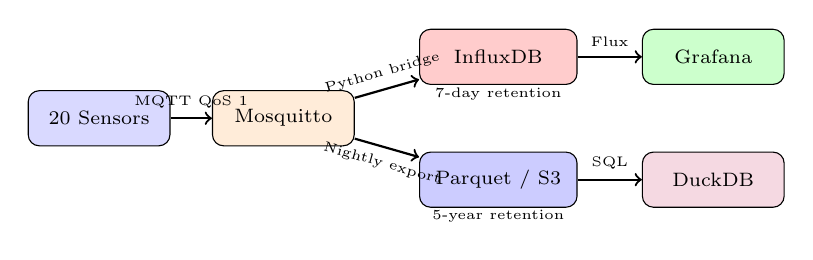
\begin{tikzpicture}[scale=0.78, every node/.style={font=\scriptsize}]
        % Sensors
        \node[draw, fill=blue!15, minimum width=1.8cm, minimum height=0.7cm, rounded corners] (sens) at (0,0) {20 Sensors};
        % Broker
        \node[draw, fill=orange!15, minimum width=1.8cm, minimum height=0.7cm, rounded corners] (mqtt) at (3,0) {Mosquitto};
        % Hot path
        \node[draw, fill=red!20, minimum width=2cm, minimum height=0.7cm, rounded corners] (influx) at (6.5,1) {InfluxDB};
        \node[font=\tiny] at (6.5,0.4) {7-day retention};
        % Cold path
        \node[draw, fill=blue!20, minimum width=2cm, minimum height=0.7cm, rounded corners] (parquet) at (6.5,-1) {Parquet / S3};
        \node[font=\tiny] at (6.5,-1.6) {5-year retention};
        % Dashboard
        \node[draw, fill=green!20, minimum width=1.8cm, minimum height=0.7cm, rounded corners] (grafana) at (10,1) {Grafana};
        % Analytics
        \node[draw, fill=purple!15, minimum width=1.8cm, minimum height=0.7cm, rounded corners] (duckdb) at (10,-1) {DuckDB};

        \draw[->, thick] (sens) -- node[above]{\tiny MQTT QoS 1} (mqtt);
        \draw[->, thick] (mqtt) -- node[above, sloped]{\tiny Python bridge} (influx);
        \draw[->, thick] (mqtt) -- node[below, sloped]{\tiny Nightly export} (parquet);
        \draw[->, thick] (influx) -- node[above]{\tiny Flux} (grafana);
        \draw[->, thick] (parquet) -- node[above]{\tiny SQL} (duckdb);
    \end{tikzpicture}
    \end{center}

    \vspace{0.1cm}
    \begin{columns}
        \column{0.5\textwidth}
        \textbf{Topic design:}\\
        \texttt{\scriptsize greenhouse/zone\{1-5\}/sensor\{1-4\}/\{temp|humidity\}}\\
        Total: 5 zones $\times$ 4 sensors $\times$ 2 metrics = \textbf{40 topics}

        \vspace{0.1cm}
        \textbf{Cost (1 year, 20 sensors at 1/min):}
        \begin{itemize}
            \item Raw points: 20 $\times$ 1440 $\times$ 365 = 10.5M/yr
            \item Parquet+Zstd: $\sim$15 MB/yr
            \item S3 cost: 15 MB $\times$ \$0.023 $\approx$ \textbf{\$0.004/year}
        \end{itemize}

        \column{0.5\textwidth}
        \textbf{Why this architecture:}
        \begin{itemize}
            \item MQTT QoS 1: greenhouse alerts must arrive
            \item InfluxDB hot path: real-time dashboard
            \item Parquet cold path: trend analysis over years
            \item Grafana: operator-friendly, no code
            \item DuckDB: ad-hoc queries on archived data
        \end{itemize}

        \vspace{0.1cm}
        \begin{exampleblock}{Scale test}
            At 10,000 sensors: Parquet $\approx$ 7.5 GB/yr. S3 cost: \textbf{\$2.07/year}. The pipeline scales linearly.
        \end{exampleblock}
    \end{columns}
\end{frame}

%==============================================================================
\section{Resources}
%==============================================================================

\begin{frame}{Datasets and References}
    \textbf{Datasets used in these exercises:}

    \vspace{0.2cm}
    \footnotesize
    \begin{center}
    \begin{tabular}{p{4cm}p{3cm}p{4cm}}
        \toprule
        \textbf{Dataset} & \textbf{Source} & \textbf{Use} \\
        \midrule
        Temperature Readings: IoT Devices & Kaggle & Primary: all exercises \\
        MQTTset & Kaggle / MDPI Sensors & MQTT protocol structure \\
        DHT11 Sensor (1-day) & Kaggle & Alternative: Arduino data \\
        ThingSpeak Public Channels & MathWorks & Live data for bonus exercises \\
        MQTT-IoT-IDS2020 & IEEE DataPort & MQTT packet analysis \\
        \bottomrule
    \end{tabular}
    \end{center}
    \normalsize

    \vspace{0.2cm}
    \textbf{Key references:}
    \begin{itemize}
        \item HiveMQ MQTT Essentials: \texttt{hivemq.com/mqtt/}
        \item InfluxDB Python Client: \texttt{github.com/influxdata/influxdb-client-python}
        \item Data Pipeline with Docker, InfluxDB, Grafana: \texttt{thedatafrog.com}
        \item Python MQTT + InfluxDB Tutorial: \texttt{influxdata.com/blog/python-mqtt-tutorial}
        \item DuckDB Documentation: \texttt{duckdb.org/docs}
    \end{itemize}
\end{frame}

\begin{frame}{Questions?}
    \begin{center}
        \Huge Questions?

        \vspace{1cm}
        \normalsize
        \textbf{Eduardo Baena}\\
        \texttt{e.baena@northeastern.edu}

        \vspace{0.5cm}
        \textit{EECE5155: Wireless Sensor Networks and the Internet of Things}\\
        Spring 2026

        \vspace{0.5cm}
        \textbf{Remember:} Sensor $\rightarrow$ MQTT $\rightarrow$ Storage $\rightarrow$ Analytics $\rightarrow$ Dashboard
    \end{center}
\end{frame}

\end{document}
